\documentclass{article}
\usepackage[margin=2.5cm, top=4cm, headheight=25pt]{geometry}
\usepackage{amsmath, amssymb, enumitem, fancyhdr, graphicx}
\usepackage[indent=20pt]{parskip}
\usepackage[hidelinks]{hyperref}
\usepackage{xcolor}
\usepackage{listings}
\usepackage{subcaption}
\usepackage{url}
\usepackage[most]{tcolorbox}
\usepackage{lastpage}

\tcbuselibrary{listingsutf8} % Support for lstlistings within tcolorbox

\newtcolorbox[auto counter, number within=section]{question}[1][]{%
    colframe=gray!80,                      % Dark gray frame
    colback=gray!5,                       % Light gray background
    coltitle=black,                        % Black title
    title=\textbf{Question~\thetcbcounter}, % Bold title
    fonttitle=\bfseries\large,             % Subtle title font size
    rounded corners,                   % Slightly more rounded corners
    boxrule=0.25mm,                         % Thinner border for a sleek look
    enhanced,                              % Enhanced box features
    attach boxed title to top left={xshift=2mm, yshift=-2mm},
    boxed title style={colframe=gray!80, colback=gray!5, boxrule=0.25mm},
    % Title styling
    #1
}

\bibliographystyle{IEEEtran}
\graphicspath{{./images/}}

% -- Custom Variables --
\def\me{Rajdeep Gill 7934493}
\def\course{ECE 4260}
\def\labsection{A01}

\def\labno{1}
\def\title{Assignment 1}

% -- Styling for code snippets --
\lstset{
    basicstyle=\ttfamily\scriptsize,           % Basic font style
    keywordstyle=\color{blue},            % Keywords color
    commentstyle=\color{gray},            % Comments color
    stringstyle=\color{teal},             % Strings color
    numbers=left,                         % Line numbers on the left
    numberstyle=\tiny\color{gray},        % Line number style
    stepnumber=1,                         % Line number step
    numbersep=10pt,                       % Space between line numbers and code
    backgroundcolor=\color{lightgray!10}, % Background color
    frame=single,                         % Adds a frame around the code
    breaklines=true,                      % Line breaking for long lines
    captionpos=b,                         % Caption position
    showspaces=false,                     % Don't show spaces
    showstringspaces=false                % Don't show spaces in strings
}
\renewcommand{\lstlistingname}{Code Snippet}

\renewcommand{\arraystretch}{1.2} % For less-ugly tables
\setlength\parindent{0pt}

%----- Samples 
% Questions:
%   \begin{question}[title=Custom Question Title]
%       Question details
%   \end{question}

% Tables:
%   \begin{table}[htbp]
%       \centering
%       \caption{Table Caption}
%       \begin{tabular}{ll}
%           \toprule
%           \textbf{Column 1} & \textbf{Column 2} \\
%           \midrule
%           Row 1 & Row 2 \\
%           Row 3 & Row 4 \\
%           \bottomrule
%       \end{tabular}
%   \end{table} 

% Figures:
%   Single figure:
%       \begin{figure}[htbp]
%           \centering
%           \includegraphics[width=0.5\textwidth]{example-image}
%           \caption{Figure Caption}
%       \end{figure}
%   Multiple figures:
%       \begin{figure}[htbp]
%           \centering
%           \begin{subfigure}[b]{0.5\textwidth}
%               \includegraphics[width=\textwidth]{example-image-a}
%               \caption{First subfigure}
%           \end{subfigure}
%           \begin{subfigure}[b]{0.5\textwidth}
%               \includegraphics[width=\textwidth]{example-image-b}
%               \caption{Second subfigure}
%           \end{subfigure}
%           \caption{Main figure}
%       \end{figure}

\begin{document}

% --------------------------------------------------------------------------------
% TITLE
% --------------------------------------------------------------------------------

\begin{center}
    \huge \title

    \vspace{2mm}
    \hrule

    \vspace{4mm}
    \large \me

    \vspace{2mm}
    \large \course~\labsection

    \vspace{2mm}
    \today
\end{center}

\vspace{4mm}

% --------------------------------------------------------------------------------
% END TITLE
% --------------------------------------------------------------------------------

\newpage


\vspace{1cm}
\newpage

\pagestyle{fancy}
\fancyhead[L]{\large Assignment \labno}
\fancyhead[R]{\large \me}

\fancyfoot[C]{Page \thepage~of~\pageref{LastPage}}

% --------------------------------------------------------------------------------
% BODY
% --------------------------------------------------------------------------------

\section{Problem 1}

\begin{enumerate}
    \item Find the Euler representation of the complex numbers $z_5, z_6$ and $z_7$.

    \begin{itemize}
        \item $z_5 = \frac{z_1}{z^*_2}$
        First, we convert $z_1$ and $z_2$ to Euler form:
        \begin{align*}
            z_1 &= \frac{5}{2} + \frac{5\sqrt{3}}{2}j \\
            |z_1| &= \sqrt{\left(\frac{5}{2}\right)^2 + \left(\frac{5\sqrt{3}}{2}\right)^2} = 5 \\
            \theta_1 &= \tan^{-1}\left(\frac{5\sqrt{3}/2}{5/2}\right) = \tan^{-1}(\sqrt{3}) = \frac{\pi}{3} \\
            \implies z_1 &= 5e^{j\frac{\pi}{3}} \\
            z^*_2 &= \sqrt{3} + j \\
            |z^*_2| &= \sqrt{\sqrt{3}^2 + 1^2} = 2 \\
            \theta_2 &= \tan^{-1}\left(\frac{1}{\sqrt{3}}\right) = \frac{\pi}{6} \\
            \implies z^*_2 &= 2e^{j\frac{\pi}{6}} \\
        \end{align*}

        Using the Euler representation of $z_1$ and $z^*_2$, we can find the Euler representation of $z_5$:
        \begin{align*}
            z_5 &= \frac{z_1}{z^*_2} = \frac{5e^{j\frac{\pi}{3}}}{2e^{j\frac{\pi}{6}}} \\
            &= \frac{5}{2}e^{j\left(\frac{\pi}{3} - \frac{\pi}{6}\right)} \\
            &= \frac{5}{2}e^{j\frac{\pi}{6}} \\
        \end{align*}

        \item $z_6 = \frac{z^*_3}{z_4}$
        \begin{align*}
            z_6 &= \frac{1+e^{jn\varphi}}{1-e^{j\varphi}} \\
        \end{align*}

        The magnitude of $z_6$:
        \begin{align*}
            |z_6| &= \left|\frac{1+e^{jn\varphi}}{1-e^{j\varphi}}\right| = \frac{\left|1+e^{jn\varphi}\right|}{\left|1-e^{j\varphi}\right|}
        \end{align*}
        And the angle is:
        \begin{align*}
            \text{arg}(z_6) &= \text{arg}(1+e^{jn\varphi}) - \text{arg}(1-e^{j\varphi}) \\
        \end{align*}

        Solving for the numerator first:
        \begin{align*}
            \left|1+e^{jn\varphi}\right| &= \left|1+cos(n\varphi)+j\sin(n\varphi)\right| \\
            &= \sqrt{(1+\cos(n\varphi))^2 + \sin^2(n\varphi)} \\
            &= \sqrt{(1+2cos(n\varphi)+\cos^2(n\varphi)) + \sin^2(n\varphi)} \\
            &= \sqrt{2+2\cos(n\varphi)} \\
        \end{align*}

        The angle of the numerator is:
        \begin{align*}
            \text{arg}(1+e^{jn\varphi}) &= \text{arg}(1+cos(n\varphi)+j\sin(n\varphi)) \\
            &= \tan^{-1}\left(\frac{\sin(n\varphi)}{1+\cos(n\varphi)}\right) \\
        \end{align*}

        Solving for the magnitude of the denominator:
        \begin{align*}
            \left|1-e^{j\varphi}\right| &= \left|1-\cos(\varphi)-j\sin(\varphi)\right| \\
            &= \sqrt{(1-\cos(\varphi))^2 + \sin^2(\varphi)} \\
            &= \sqrt{(1-2\cos(\varphi)+\cos^2(\varphi)) + \sin^2(\varphi)} \\
            &= \sqrt{2-2\cos(\varphi)} \\
        \end{align*}

        The angle of the denominator is:
        \begin{align*}
            \text{arg}(1-e^{j\varphi}) &= \text{arg}(1-\cos(\varphi)-j\sin(\varphi)) \\
            &= \tan^{-1}\left(\frac{-\sin(\varphi)}{1-\cos(\varphi)}\right) \\
        \end{align*}

        The overall magnitude is:
        \begin{align*}
            |z_6| &= \frac{\sqrt{2+2\cos(n\varphi)}}{\sqrt{2-2\cos(\varphi)}} \\
            &= \sqrt{\frac{1+\cos(n\varphi)}{1-\cos(\varphi)}}
        \end{align*}

        And the angle is:
        \begin{align*}
            \theta_{z_6} = \text{arg}(z_6) &= \tan^{-1}\left(\frac{\sin(n\varphi)}{1+\cos(n\varphi)}\right) - \tan^{-1}\left(\frac{-\sin(\varphi)}{1-\cos(\varphi)}\right) \\
            &= \tan^{-1}\left(\frac{\sin(n\varphi)}{1+\cos(n\varphi)}\right) + \tan^{-1}\left(\frac{\sin(\varphi)}{1-\cos(\varphi)}\right) 
        \end{align*}

        To simplify the argument, we can use the following identities:
        \begin{align*}
            \frac{\sin(x)}{1+\cos(x)} &= \tan\left(\frac{x}{2}\right) \\
            \frac{\sin(x)}{1-\cos(x)} &= \cot\left(\frac{x}{2}\right) \\
            \cot(x) &= \tan\left(\frac{\pi}{2} - x\right) \\
        \end{align*}

        The first term becomes:
        \begin{align*}
            \tan^{-1}\left(\frac{\sin(n\varphi)}{1+cos(n\varphi)}\right) = \tan^{-1}\left(\tan\left(\frac{n\varphi}{2}\right)\right) &= \frac{n\varphi}{2}
        \end{align*}

        The second term becomes:
        \begin{align*}
            \tan^{-1}\left(\frac{\sin(\varphi)}{1-\cos{\varphi}}\right) &= \tan^{-1}\left(\cot\left(\frac{\varphi}{2}\right)\right) \\
            &= \tan^{-1}\left(\tan\left(\frac{\pi}{2} - \frac{\varphi}{2}\right)\right) \\
            &= \frac{\pi}{2} - \frac{\varphi}{2}
        \end{align*}

        The simplified argument is:
        \begin{align*}
            \theta_{z_6} = \frac{n\varphi}{2} + \frac{\pi}{2} - \frac{\varphi}{2} = \frac{(n-1)\varphi}{2} + \frac{\pi}{2}
        \end{align*}

        In polar form, $z_6$ is:
        \begin{align*}
            z_6 = \sqrt{\frac{1+\cos(n\varphi)}{1-\cos(\varphi)}}e^{j\theta_{z_6}}
        \end{align*}

        \item $z_7 = z_5z^*_6$

        \begin{align*}
            z_7 &= \frac{5}{2}e^{j\frac{\pi}{6}} \cdot \sqrt{\frac{1+\cos(n\varphi)}{1-\cos(\varphi)}}e^{-j\theta_{z_6}} \\
            &= \frac{5}{2}\sqrt{\frac{1+\cos(n\varphi)}{1-\cos(\varphi)}}e^{j\left(\frac{\pi}{6} - \frac{(n-1)\varphi}{2} - \frac{\pi}{2}\right)} \\
            &= \frac{5}{2}\sqrt{\frac{1+\cos(n\varphi)}{1-\cos(\varphi)}}e^{-j\left(\frac{\pi}{3} + \frac{(n-1)\varphi}{2}\right)} \\
        \end{align*}
    \end{itemize}

    \item Find the real and imaginary parts of $z^*_7$.
    We can convert from Euler form to rectangular form to easily find the real and imaginary parts of $z^*_7$:
    \begin{align*}
        z^*_7 &=  \frac{5}{2}\sqrt{\frac{1+\cos(n\varphi)}{1-\cos(\varphi)}}e^{j\left(\frac{\pi}{3} + \frac{(n-1)\varphi}{2}\right)} \\
        &= \frac{5}{2}\sqrt{\frac{1+\cos(n\varphi)}{1-\cos(\varphi)}}\left(\cos\left(\frac{\pi}{3} + \frac{(n-1)\varphi}{2}\right) + j\sin\left(\frac{\pi}{3} + \frac{(n-1)\varphi}{2}\right)\right) \\
    \end{align*}

    This gives us the result:
    \begin{align*}
        \text{Re}(z^*_7) &= \frac{5}{2}\sqrt{\frac{1+\cos(n\varphi)}{1-\cos(\varphi)}}\cos\left(\frac{\pi}{3} + \frac{(n-1)\varphi}{2}\right) \\
        \text{Im}(z^*_7) &= \frac{5}{2}\sqrt{\frac{1+\cos(n\varphi)}{1-\cos(\varphi)}}\sin\left(\frac{\pi}{3} + \frac{(n-1)\varphi}{2}\right) \\
    \end{align*}
\end{enumerate}

\section{Problem 2}

\begin{itemize}
    \item $g_1(t) = g(-t)$
    \item $g_2(t) = g_1(t-1) + g(t-1) = g(-t+1) + g(t-1)$
    \item $g_3(t) = g_1(t+1) + g(t-1) = g(-t-1) + g(t-1)$
    \item $g_4(t) = g_1(t+1/2) + g(t-1/2) = g(-t-1/2) + g(t-1/2)$
    \item $g_5(t) = \frac{3}{2}g(\frac{t}{2}-1)$
\end{itemize}
\newpage
\section{Problem 3}
\autoref{fig:p1} shows the original signal $g(t)$ and the three transformed signals $g_1(t), g_2(t)$ and $g_3(t)$. The code to generate the signals is shown in \autoref{code:p3}
\begin{figure}[ht!]
    \centering
    \begin{subfigure}{\textwidth}
        \centering
        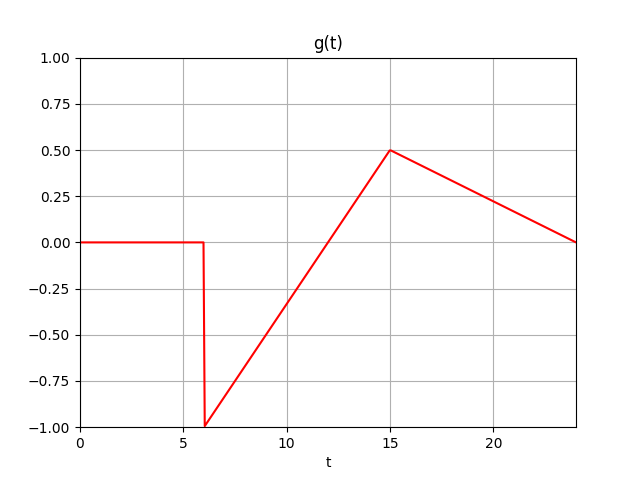
\includegraphics[width=0.5\textwidth]{p1_1.png}
        \caption{Original Signal $g(t)$}
    \end{subfigure}
    \newline
    \begin{subfigure}{0.3\textwidth}
        \centering
        
\includegraphics[width=\textwidth]{p1_2.png}
        \caption{$g_1(t) = g(3t)$}
    \end{subfigure}
    \begin{subfigure}{0.3\textwidth}
        \centering
        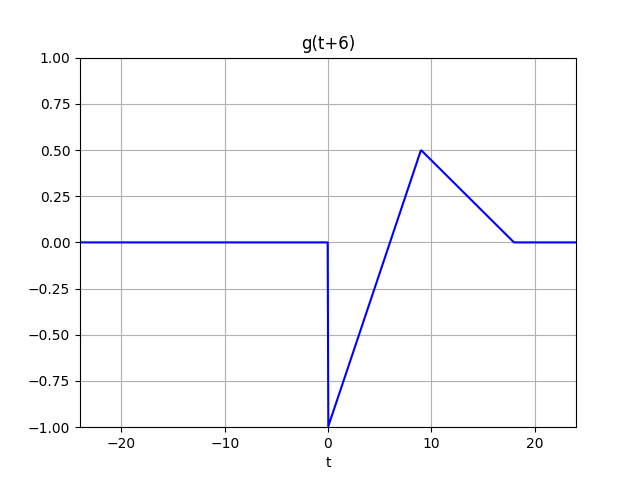
\includegraphics[width=\textwidth]{p1_3.png}
        \caption{$g_2(t) = g(t+6)$}
    \end{subfigure}
    \begin{subfigure}{0.3\textwidth}
        \centering
        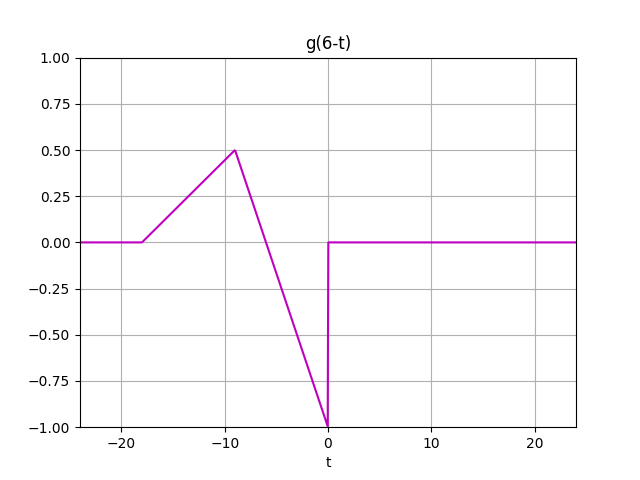
\includegraphics[width=\textwidth]{p1_4.png}
        \caption{$g_3(t) = g(6-t)$}
    \end{subfigure}
    \caption{Graphs of the original signal and the transformed signals}
    \label{fig:p1}
\end{figure}

\begin{lstlisting}[language=Python, caption={Python code to generate the signals}, label={code:p3}]
import numpy as np
def g(t):
    if t > 6 and t <= 15:
        return 1/6 * t - 2
    elif t > 15 and t <= 24:
        return -1/18 * t + 4/3
    else:
        return 0
t = np.linspace(-30, 30, 1000)
g0 = [g(i) for i in t]
g1 = [g(3*i) for i in t]
g2 = [g(i+6) for i in t]
g3 = [g(6-i) for i in t]
\end{lstlisting}

\section{Problem 4}
Since the signal is periodic, we can find the average power of the entire signal by integrating over 1 period and dividing by the period. The average power is given by:
\[
    P_g(t) = \frac{1}{T} \int_{T} |g(t)|^2 dt
\]

The period of this signal is $T = 4$ and we can integrate from -2 to 2.
\begin{align*}
    P_g(t) &= \frac{1}{4} \int_{-2}^{2} |g(t)|^2 dt \\
    &= \frac{1}{4} \int_{-2}^{2} (t^3)^2 dt = \frac{1}{4} \int_{-2}^{2} t^6 dt \\
    &= \frac{1}{4} \left[\frac{t^7}{7}\right]_{-2}^{2} = \frac{1}{4} \left[\frac{128}{7} - \frac{-128}{7}\right] \\
    &= \frac{1}{4} \left[\frac{256}{7}\right] = \boxed{\frac{64}{7}} \\
\end{align*}

\section{Problem 5}
\begin{enumerate}[label=5.\arabic*]
    \item Show that $\mathcal{H}[.]$ is linear.
    To show that $\mathcal{H}[.]$ is linear, we need to show that it satisfies both the additivity and homogeneity properties.

    Additivity:

    Let $x_1(t)$ and $x_2(t)$ be two signals. Then, with $h(t)$ a fixed signal, we have:

    \begin{align*}
        x_1(t) \rightarrow y_1(t) &= \mathcal{H}[x_1(t)] = x_1(t) h(t) \\
        x_2(t) \rightarrow y_2(t) &= \mathcal{H}[x_2(t)] = x_2(t) h(t) \\
        (x_1(t) + x_2(t)) \rightarrow y_3(t) &= \mathcal{H}[x_1(t) + x_2(t)] = (x_1(t) + x_2(t)) h(t) \\
        &= x_1(t)h(t) + x_2(t)h(t) = y_1(t) + y_2(t) \\
    \end{align*}

    Thus $\mathcal{H}[.]$ satisfies the additivity property.

    Homogeneity:

    Let $x(t)$ be a signal and $a$ be a scalar. Then, with $h(t)$ a fixed signal, we have:

    \begin{align*}
        x(t) \rightarrow y_1(t) &= \mathcal{H}[x(t)] = x(t) h(t) \\
        ax(t) \rightarrow y_2(t) &= \mathcal{H}[ax(t)] = ax(t) h(t) \\
        &= a(x(t)h(t)) = ay_1(t) \\
    \end{align*}

    Thus $\mathcal{H}[.]$ satisfies the homogeneity property and is linear.

    \item Show that if $\mathcal{H}[.]$ is time-invariant, then h(t) must be a constant, i.e. $h(t) = c, \forall t, c \in \mathbb{R}$.
    
    A system is time-invariant if a shift in the input signal results in a corresponding shift in the output signal. Let $x(t)$ be a signal.
    \begin{align*}
        x(t-t_0) \rightarrow y_1(t) &= \mathcal{H}[x(t-t_0)] = x(t-t_0) h(t) \\
        y_2(t-t_0) &= x(t-t_0) h(t-t_0) \\
    \end{align*}
    Then, $y_2(t-t_0) = y_1(t)$ if, and only if, $h(t) = c$ for some constant $c$. If $h(t) = c$, then $y_1(t) = cx(t-t_0)$ and $y_2(t-t_0) = cx(t-t_0)$. 
    \item Suppose that the switch is closed for $-1/2 \leq t \leq 1/2$. Using 5.1, show that this is a linear system.

    The new system is given by:
    \[
       \mathcal{H}[x(t)] =\begin{cases}
        x(t) & \text{if } -\frac{1}{2} \leq t \leq \frac{1}{2} \\
        0 & \text{otherwise}
        \end{cases}
    \]

    Let $x_1(t)$ and $x_2(t)$ be two signals. Then we have:
    \begin{align*}
        \mathcal{H}[x_1(t) + x_2(t)] &= \begin{cases}
            x_1(t) + x_2(t) & \text{if } -\frac{1}{2} \leq t \leq \frac{1}{2} \\
            0 & \text{otherwise}
        \end{cases} \\
        &= \begin{cases}
            x_1(t) & \text{if } -\frac{1}{2} \leq t \leq \frac{1}{2} \\
            0 & \text{otherwise}
        \end{cases} + \begin{cases}
            x_2(t) & \text{if } -\frac{1}{2} \leq t \leq \frac{1}{2} \\
            0 & \text{otherwise}
        \end{cases} \\
        &= \mathcal{H}[x_1(t)] + \mathcal{H}[x_2(t)]
    \end{align*}

    And:
    \begin{align*}
        \mathcal{H}[ax(t)] &= \begin{cases}
            ax(t) & \text{if } -\frac{1}{2} \leq t \leq \frac{1}{2} \\
            0 & \text{otherwise}
        \end{cases} \\
        &= a\begin{cases}
            x(t) & \text{if } -\frac{1}{2} \leq t \leq \frac{1}{2} \\
            0 & \text{otherwise}
        \end{cases} \\
        &= a\mathcal{H}[x(t)]
    \end{align*}

    Thus the system satisfies the additivity and homogeneity properties and is linear.

    \item Suppose that the switch is turned on and off at various time intervals. Is the system still linear any why? Is it time-invariant and why?

    We can represent the new system as:
    \[
        \mathcal{H}[x(t)] =\begin{cases}
        x(t) & \text{if } t \in \bigcup_{i=1}^{n} [a_i, b_i] \\
        0 & \text{otherwise}
        \end{cases}
    \]

    We can show that it is linear as it follows both additivity and homogeneity:
    \begin{align*}
        \mathcal{H}[ax_1(t) +bx_2(t)] &= \begin{cases}
            ax_1(t) + bx_2(t) & \text{if } t \in \bigcup_{i=1}^{n} [a_i, b_i] \\
            0 & \text{otherwise}
        \end{cases} \\
        &= a\begin{cases}
            x_1(t) & \text{if } t \in \bigcup_{i=1}^{n} [a_i, b_i] \\
            0 & \text{otherwise}
        \end{cases} + b\begin{cases}
            x_2(t) & \text{if } t \in \bigcup_{i=1}^{n} [a_i, b_i] \\
            0 & \text{otherwise}
        \end{cases} \\
        &= a\mathcal{H}[x_1(t)] + b\mathcal{H}[x_2(t)]
    \end{align*}

    It is not time-invariant as the output signal will change depending on the time intervals the switch is on or off. A delay in the input signal will not result in a corresponding delay in the output signal. 
    \begin{align*}
        x(t-t_0) \rightarrow y_1(t) &= \mathcal{H}[x(t-t_0)] = \begin{cases}
            x(t-t_0) & \text{if } t \in \bigcup_{i=1}^{n} [a_i, b_i] \\
            0 & \text{otherwise}
        \end{cases} \\
        y_2(t-t_0) &= \begin{cases}
            x(t-t_0) & \text{if } (t-t_0) \in \bigcup_{i=1}^{n} [a_i, b_i] \\
            0 & \text{otherwise}
        \end{cases} \\
    \end{align*}
    We see that adding a delay in the output also adds a delay to the time-intervals, unlike the delayed input signal, where it is on and off at fixed intervals. 
    
    For example, if the switch is on for $[2, 3] \cup [5, 6]$, a delay in the input will result in the portion of the signal being on between these two values, where as a delay in the output will result in the signal being on for $[2+t_0, 3+t_0] \cup [5+t_0, 6+t_0]$.


    \item Suppose that the switch is turned on at $t=0$ and stays on forever. Is the system now linear and why? Is it time-invariant and why?

    We can define the new system as:
    \begin{align*}
        y(t) = \mathcal{H}[x(t)] &= u(t)x(t) \\
        u(t) &= \begin{cases}
            1 & \text{if } t \geq 0 \\
            0 & \text{otherwise}
        \end{cases}
    \end{align*}

    The system is linear as it satisfies both additivity and homogeneity:
    \begin{align*}
        y(ax_1(t) + bx_2(t)) = \mathcal{H}[ax_1(t) + bx_2(t)] &= u(t)(ax_1(t) + bx_2(t)) \\
        &= au(t)x_1(t) + bu(t)x_2(t) \\
        &= a\mathcal{H}[x_1(t)] + b\mathcal{H}[x_2(t)] \\
        &= ay_1(t) + by_2(t)
    \end{align*}

    It is not time-invariant and we can show this by considering a delay in the input signal:
    \begin{align*}
        x(t-t_0) \rightarrow y_1(t) &= u(t)x(t-t_0) \\
        y_2(t-t_0) &= u(t-t_0)x(t-t_0) \\
        &\neq y_1(t)
    \end{align*}

    Therefore, since a delay in the input does not lead to the same result as a delay in the output, the system is not time-invariant.

\end{enumerate}



% --------------------------------------------------------------------------------
% END BODY
% --------------------------------------------------------------------------------

\end{document}
